\subsubsection{Stufenindexprofil}

Bei polymer optischen Fasern mit Stufenindexprofil (SI-POF) steigt die Brechzahl
beim Übergang vom Mantel zum Kern abrupt an (linke Grafik in
\autoref{fig:pofsi}). Dies führt zu der schon erwähnten Totalreflexion an der
Kerngrenze (rechte Grafik in \autoref{fig:pofsi}).

Als Kernmaterial wird Polymethylmethacrylat mit einem Durchmesser von ca. 1 mm
eingesetzt, welches von einem ca. 10 µm dicken Mantel umgeben ist
\cite{pofacsi}. Alternativ kommen auch Polystyrol und Polycarbonat zum Einsatz,
jedoch sind sie für die Datenübertragung aufgrund ihrer geringeren optischen
Qualität weniger geeignet.

Beim Stufenindexprofil werden Durchsatzraten von ca. 100 Megabit/s auf 100 m
erreicht.

\ifthenelse{\boolean{showPics}}{
    \begin{figure}[h]
        \begin{center}
            \begin{minipage}[t]{0.4\textwidth}
                \begin{center}
                    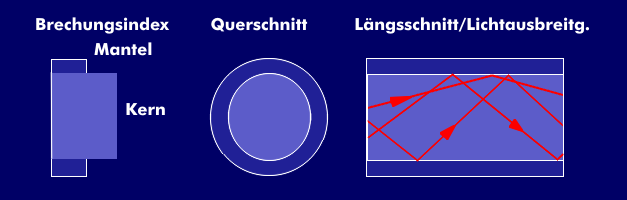
\includegraphics[width=0.9\textwidth]{Bilder/Optische_Wellenleiter_Die_Polymer_Optische_Faser/Brechzahlprofile/pofsi.png}
                    \caption[Aufbau einer SI-POF \newline \url{http://www.itwissen.info/bilder/aufbau-und-brechungsprofil-der-stufenindex-profilfaser.png} (zuletzt aufgerufen am 19.09.2015)]{Aufbau einer SI-POF}
                    \label{fig:pofsi}
                \end{center}
            \end{minipage}
            \hspace{0.025\textwidth}
            \begin{minipage}[t]{0.4\textwidth}
                \begin{center}
                    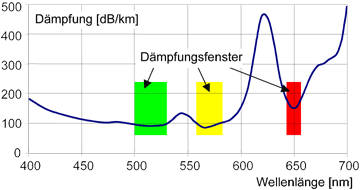
\includegraphics[height=0.1\textheight]{Bilder/Optische_Wellenleiter_Die_Polymer_Optische_Faser/Funktionsweise/pofdaempfung.png}
                    \caption[Dämpfungsfenster bei einer SI-POF \newline \url{http://www.pofac.fh-nuernberg.de/pofac/de/was_sind_pof/images/pmma_daempfung.png} (zuletzt aufgerufen am 19.09.2015)]{Dämpfungsfenster bei einer SI-POF}
                    \label{fig:pofdaempfung}
                \end{center}
            \end{minipage}
        \end{center}
    \end{figure}
}{}

Die Dämpfungsfenster einer polymer optischen Faser mit Stufenindexprofil liegen
bei den Farben grün, gelb und rot (\autoref{fig:pofdaempfung}). Um die
Intensitätsabnahme möglichst gering zu halten und damit die Reichweite zu
erhöhen werden Wellenlängen für die Lichtimpulse gewählt, die in den
Dämpfungsfenstern liegen. Als Lichtquelle kann zum Beispiel eine LED verwendet
werden, als Empfänger kommen Photodetektoren zum Einsatz. Der geringe Preis und
die robuste Übertragung auf kurzen Strecken machen die SI-POF zu einer beliebten
Alternative gegenüber Kupferkabeln in Industrieanlagen und in Fahrzeugen.
\cite{poflee}
